% ======================================================================
%  Punto 1.2 (tercera versión).
%  Reemplaza por completo el archivo punto_1_2_cuerpo.tex anterior.
%  Usa las macros y colores del bloque del taller (\bk, \destacado,
%  \Real, \Imag, definicionT, observacionT, ondaT, colCu, colSu, colSd,
%  resaltado) y cita ecuaciones del punto 1.1, así que va después de él.
%  Cada vez que se cita una ecuación, también se escribe en el texto.
% ======================================================================

El widget está publicado como página web en
\url{https://mariasaurius.github.io/taller1-computacion-cuantica/}, y su código, junto con la
versión en Python (Jupyter), está en el repositorio
\url{https://github.com/mariasaurius/taller1-computacion-cuantica}. La
figura~\ref{fig:widget} muestra sus tres paneles para el estado
$\alpha=\frac1{\sqrt2}$, $\beta=\frac1{\sqrt2}e^{i\pi/3}$, que se usa como ejemplo a lo largo de
toda la solución.

\begin{figure}[htbp]
\centering
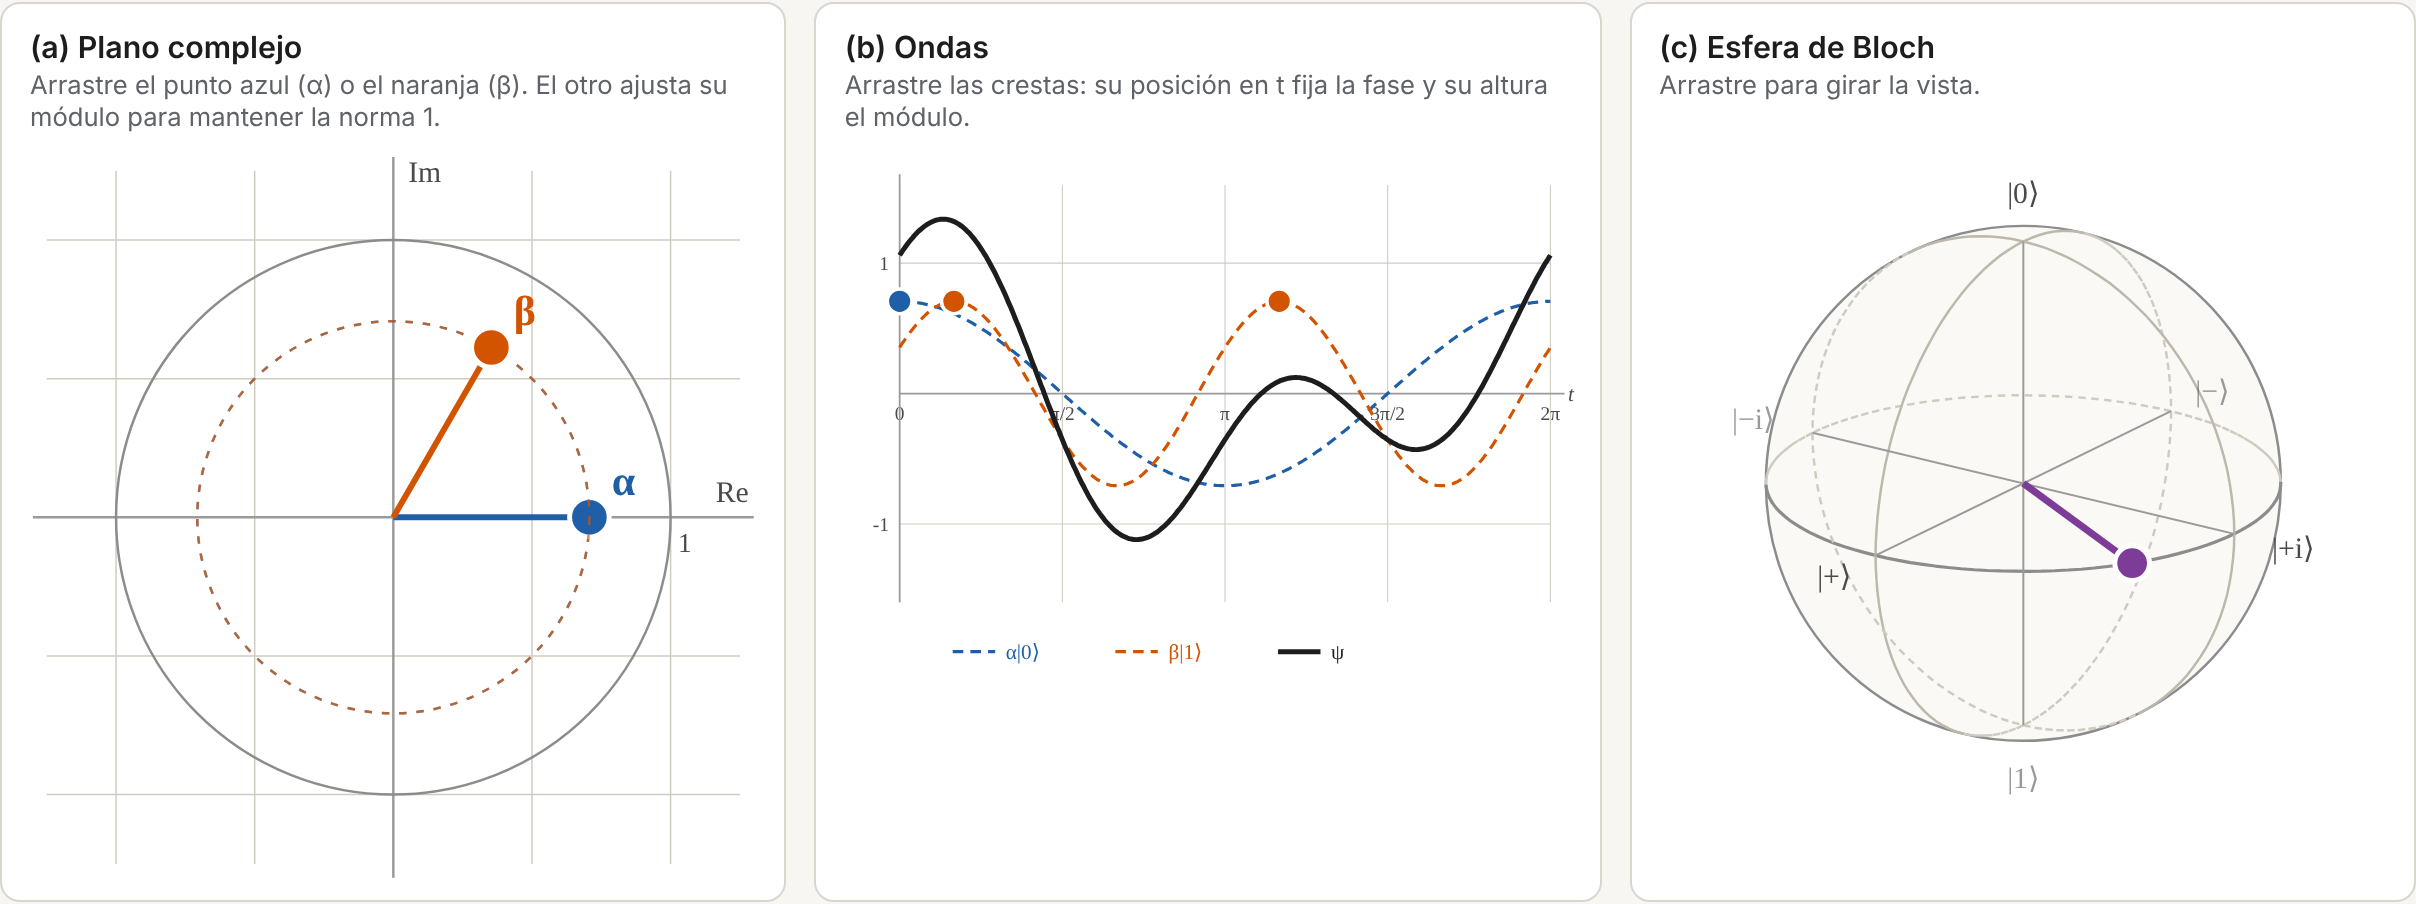
\includegraphics[width=\linewidth]{Imágenes/widget_punto_1_2.png}
\caption{Los tres paneles del widget para $\alpha=\frac1{\sqrt2}$,
$\beta=\frac1{\sqrt2}e^{i\pi/3}$. En (a) se arrastran los coeficientes, en (b) las crestas de las
ondas y en (c) se gira la esfera; los tres paneles se actualizan a la vez.}
\label{fig:widget}
\end{figure}

%======================================================================
\subsection*{El estado \texorpdfstring{$\ket\psi$}{psi}}
%======================================================================

El objeto que muestran los tres paneles es un estado de un qubit en el espacio $V$ del
punto~1.1. Allí se vio, en la ecuación~$f=\alpha\cdot\cos t+\beta\cdot\cos 2t$ \eqref{eq:alfa-beta}, que todo elemento de $V$ se escribe
como
\[
  f=\alpha\cdot\cos t+\beta\cdot\cos 2t=\alpha\ket0+\beta\ket1,\qquad \alpha,\beta\in\mathbb C,
\]
y que esta escritura es única: por el lema~\ref{lema:independencia}, las funciones $\cos t$,
$\sin t$, $\cos 2t$ y $\sin 2t$ son linealmente independientes, de modo que dos expresiones que
dan la misma función tienen los mismos coeficientes. También se vio, en la
ecuación~$\bk fg=\overline\alpha\,\alpha'+\overline\beta\,\beta'$ \eqref{eq:hermitico-coord}, que el producto hermítico de
$f=\alpha\ket0+\beta\ket1$ y $g=\alpha'\ket0+\beta'\ket1$ es
\[
  \bk fg=\overline\alpha\,\alpha'+\overline\beta\,\beta' ,
\]
así que la norma al cuadrado de $f$ es $\bk ff=\overline\alpha\alpha+\overline\beta\beta
=|\alpha|^2+|\beta|^2$.

\begin{definicionT}[Estado de un qubit]
Un \emph{estado} de un qubit es un vector de $V$ de norma $1$,
\begin{equation}\label{eq:estado}
  \ket\psi=\alpha\ket0+\beta\ket1,\qquad \alpha,\beta\in\mathbb C,\qquad |\alpha|^2+|\beta|^2=1 .
\end{equation}
Los números $\alpha$ y $\beta$ se llaman \emph{coeficientes} o \emph{amplitudes} del estado. Al
medir el qubit en la base $\{\ket0,\ket1\}$ se obtiene el resultado $0$ con probabilidad
$|\alpha|^2$ y el resultado $1$ con probabilidad $|\beta|^2$ (regla de Born); la condición
$|\alpha|^2+|\beta|^2=1$ dice que estas dos probabilidades suman $1$.
\end{definicionT}

El widget trabaja siempre con estados: cuando se modifica uno de los coeficientes, el otro
ajusta su módulo para que se siga cumpliendo $|\alpha|^2+|\beta|^2=1$.

\paragraph{Los coeficientes en forma polar.}
La regla de multiplicación del enunciado,
\[
  (Ae^{ix})\cdot\cos nt=A\cos(nt-x),
\]
está escrita en términos de la forma polar de un número complejo. Para aplicarla a $\alpha$ y a
$\beta$ es necesario escribirlos de esa manera, y por eso en esta solución se usan las mismas
letras del enunciado.

\begin{definicionT}[Módulos y fases de los coeficientes]
Los coeficientes del estado $\ket\psi=\alpha\ket0+\beta\ket1$ se escriben en forma polar como
\begin{equation}\label{eq:polar-ab}
  \destacado{\alpha=A\,e^{ix},\qquad \beta=B\,e^{iy},\qquad A,B\ge 0,\quad x,y\in\mathbb R .}
\end{equation}
Los números $A=|\alpha|$ y $B=|\beta|$ son los \emph{módulos} de los coeficientes y los ángulos
$x$ y $y$ son sus \emph{fases}. La condición de norma $1$ se escribe $A^2+B^2=1$. Como $e^{ix}$
no cambia al sumar $2\pi$ a $x$, las fases están determinadas salvo múltiplos enteros de $2\pi$;
las igualdades entre fases se entienden en ese sentido y se escriben con el símbolo $\equiv$: para dos ángulos $a$ y $b$, la notación $a\equiv b\pmod{2\pi}$ significa que $a-b$ es un múltiplo entero de $2\pi$, es decir, que $a$ y $b$ representan el mismo ángulo. La abreviatura ``mód'' viene de ``módulo $2\pi$'' y no tiene relación con el módulo $|\alpha|$ de un número complejo. Cuando no hay confusión se escribe solo $a\equiv b$. Si
$A=0$, entonces $\alpha=0$ para cualquier valor de $x$, y la fase $x$ no está determinada (lo
mismo ocurre con $y$ si $B=0$).
\end{definicionT}

En el estado del ejemplo, $\alpha=\frac1{\sqrt2}=\frac1{\sqrt2}e^{i0}$ y
$\beta=\frac1{\sqrt2}e^{i\pi/3}$, de modo que
\[
  A=B=\tfrac1{\sqrt2},\qquad x=0,\qquad y=\tfrac\pi3 .
\]

%======================================================================
\subsection*{Las tres representaciones del estado}
%======================================================================

Los tres paneles no muestran tres objetos distintos sino el mismo estado $\ket\psi$ descrito de
tres maneras. Cada una usa un tipo de objeto matemático diferente.

\paragraph{Panel (a): dos números complejos.}
En el panel (a), el estado se describe por la pareja de coeficientes $(\alpha,\beta)$. Cada
coeficiente es un número complejo y se dibuja como un punto del plano complejo: el módulo ($A$ o
$B$) es la distancia del punto al origen y la fase ($x$ o $y$) es el ángulo que forma el segmento
que lo une con el origen, medido desde el eje real (figura~\ref{fig:a-b}, izquierda). Como
$A^2+B^2=1$, ambos puntos están dentro del círculo de radio $1$, y si uno se aleja del origen el
otro tiene que acercarse.

\paragraph{Panel (b): una función, es decir, una onda.}
En el panel (b), el estado se describe por lo que es como elemento de $V$: una función
$\psi\colon[0,2\pi]\to\mathbb R$. Según la sección siguiente, esa función es la suma de dos
ondas, una de frecuencia $1$, que proviene de $\alpha\ket0$, y otra de frecuencia $2$, que
proviene de $\beta\ket1$ (figura~\ref{fig:a-b}, derecha). En este contexto, \emph{onda} significa
una función de la forma $A\cos(nt-x)$: una curva que oscila entre $-A$ y $A$ y que completa $n$
oscilaciones en $[0,2\pi]$.

\paragraph{Panel (c): un punto de una esfera.}
En el panel (c), el estado se describe por un punto $\vec r=(r_x,r_y,r_z)\in\mathbb R^3$ de la
esfera de radio $1$ centrada en el origen, llamada esfera de Bloch. Este punto no guarda toda la
información del estado, sino solo la que tiene significado físico; la parte que descarta es la
fase global, que se define más adelante.

\medskip
La tabla siguiente resume las tres descripciones y cuántos números reales usa cada una.
\[
\renewcommand{\arraystretch}{1.35}
\begin{array}{l|l|l}
\text{Panel} & \text{Objeto} & \text{Números reales que lo determinan}\\ \hline
\text{(a) coeficientes} & (\alpha,\beta)\in\mathbb C^2 & A,\ x,\ B,\ y\ \ (\text{con } A^2+B^2=1)\\
\text{(b) onda} & \psi(t)=A\cos(t-x)+B\cos(2t-y) & \text{los mismos } A,\ x,\ B,\ y\\
\text{(c) esfera} & \vec r\in\mathbb R^3,\ \lVert\vec r\rVert=1 & \text{dos ángulos } \theta,\ \varphi
\end{array}
\]
Las descripciones (a) y (b) contienen exactamente la misma información, porque cada pareja
$(\alpha,\beta)$ corresponde a una única función de $V$ y viceversa (por la unicidad de los
coeficientes recordada al comienzo); pasar de una a la otra es una traducción que no pierde
nada. En cambio, la descripción (c) usa un número menos: al pasar a la esfera se pierde la fase
global, y al volver de la esfera hay que elegirla. La figura~\ref{fig:mapa} resume las seis
traducciones, y al final de la solución se reúnen todas sus fórmulas.

\begin{figure}[htbp]
\centering
\begin{tikzpicture}[
  caja/.style={draw=#1, very thick, rounded corners=2mm, fill=#1!6,
               align=center, minimum width=4.4cm, minimum height=1.45cm, font=\small},
  flecha/.style={-{Stealth[length=2.5mm]}, thick, black!70},
  etq/.style={font=\footnotesize, align=center, fill=white, inner sep=1.5pt}
]
  \node[caja=colCu] (a) at (0,0)    {\textbf{(a) Coeficientes}\\[1pt]
        $\alpha=Ae^{ix},\ \beta=Be^{iy}$};
  \node[caja=colSu] (b) at (8.2,0)  {\textbf{(b) Onda}\\[1pt]
        $\psi(t)=A\cos(t-x)+B\cos(2t-y)$};
  \node[caja=colSd] (c) at (4.1,-4) {\textbf{(c) Esfera de Bloch}\\[1pt]
        $\vec r=(\sin\theta\cos\varphi,\,\sin\theta\sin\varphi,\,\cos\theta)$};
  % (a) <-> (b)
  \draw[flecha] ([yshift=3mm]a.east) -- node[etq, above=1pt]{regla del enunciado \eqref{eq:a-b}}
        ([yshift=3mm]b.west);
  \draw[flecha] ([yshift=-3mm]b.west) -- node[etq, below=1pt]{lectura de las crestas \eqref{eq:b-a}} ([yshift=-3mm]a.east);
  % (a) <-> (c)
  \draw[flecha] ([xshift=-8mm]a.south) -- ([xshift=-14mm]c.north);
  \draw[flecha] ([xshift=-6mm]c.north) -- ([xshift=0mm]a.south);
  \node[etq, anchor=east] at (0.15,-2.05) {$\downarrow$ se olvida la fase global \eqref{eq:theta}, \eqref{eq:phi}\\
        $\uparrow$ se elige la fase global $\gamma$ \eqref{eq:c-a}};
  % (b) <-> (c)
  \draw[flecha] ([xshift=0mm]b.south) -- ([xshift=6mm]c.north);
  \draw[flecha] ([xshift=14mm]c.north) -- ([xshift=8mm]b.south);
  \node[etq, anchor=west] at (8.0,-2.05) {$\downarrow$ se olvida la fase global \eqref{eq:b-c}\\
        $\uparrow$ se elige la fase global $\gamma$ \eqref{eq:c-b}};
\end{tikzpicture}
\caption{Las tres representaciones del estado $\ket\psi$ y las fórmulas que traducen entre
ellas. Entre (a) y (b) la traducción no pierde información; hacia (c) se pierde la fase global
$\gamma$, y desde (c) hay que elegirla.}
\label{fig:mapa}
\end{figure}

%======================================================================
\subsection*{De los coeficientes a la onda: del panel (a) al panel (b)}
%======================================================================

\paragraph{Qué se traduce.}
Se parte de dos números complejos, $\alpha$ y $\beta$, y se quiere obtener la función
$\psi(t)$ que representan. No se trata solo de cambiar la escritura de $\alpha$ y $\beta$ a forma
polar: la forma polar es la herramienta que permite aplicar la regla del enunciado, y el
resultado de aplicarla es una función de $t$, no otro número.

\paragraph{Fórmula.}
El estado es la suma de $\alpha\ket0=\alpha\cdot\cos t$ y $\beta\ket1=\beta\cdot\cos 2t$. Al
aplicar la regla del enunciado, $(Ae^{ix})\cdot\cos nt=A\cos(nt-x)$, con $\alpha=Ae^{ix}$ y
$n=1$, y luego con $\beta=Be^{iy}$ y $n=2$, se obtienen las dos ondas que componen el estado; al
sumarlas se obtiene la función completa:
\begin{equation}\label{eq:a-b}
  \destacado{\alpha\ket0=A\cos(t-x),\qquad \beta\ket1=B\cos(2t-y),\qquad
  \psi(t)=A\cos(t-x)+B\cos(2t-y).}
\end{equation}
Si se prefiere la forma rectangular $\alpha=a_1+ib_1$, $\beta=a_2+ib_2$, la
fórmula~$(a+ib)\cdot\cos nt=a\cos nt+b\sin nt$ \eqref{eq:regla-coef} del punto~1.1, $(a+ib)\cdot\cos nt=a\cos nt+b\sin nt$, da la
misma función escrita como $\psi(t)=a_1\cos t+b_1\sin t+a_2\cos 2t+b_2\sin 2t$. La forma polar
tiene la ventaja de que cada número se lee directamente en la gráfica.

\paragraph{Qué significa.}
El módulo de cada coeficiente es la altura de su onda y la fase es cuánto se corre la onda hacia
la derecha. Para ubicar ese corrimiento en la gráfica se sigue la posición de las crestas.

\begin{definicionT}[Cresta]
Una \emph{cresta} de una onda $A\cos(nt-x)$ con $A>0$ es un punto donde la onda alcanza su valor
máximo, $A$. Como $\cos u=1$ exactamente cuando $u$ es un múltiplo entero de $2\pi$, las crestas
son los valores de $t$ con $nt-x=2\pi k$, $k\in\mathbb Z$, es decir, $t=\frac xn+\frac{2\pi k}n$.
\end{definicionT}

La onda $\alpha\ket0=A\cos(t-x)$, de frecuencia $1$, tiene una sola cresta en $[0,2\pi)$, en
$t_\alpha\equiv x$, con altura $A$. La onda $\beta\ket1=B\cos(2t-y)$, de frecuencia $2$, tiene
dos, separadas por $\pi$: la primera en $t_\beta\equiv\frac y2$ y la segunda en $t_\beta+\pi$,
ambas con altura $B$. La fase $y$ se divide entre $2$ porque esa onda oscila el doble de rápido:
un ángulo $y$ corresponde a un corrimiento de solo $y/2$ unidades en $t$. En el ejemplo,
$t_\alpha=0$ y $t_\beta=\frac\pi6$ (figura~\ref{fig:a-b}).

\begin{figure}[htbp]
\centering
\begin{tikzpicture}[scale=1.25, line cap=round]
  \draw[black!15] (-1.25,-1.25) grid[step=0.5] (1.25,1.25);
  \draw[-{Stealth[length=2mm]}, black!60] (-1.35,0) -- (1.45,0) node[right, font=\footnotesize]{Re};
  \draw[-{Stealth[length=2mm]}, black!60] (0,-1.35) -- (0,1.45) node[above, font=\footnotesize]{Im};
  \draw[black!55] (0,0) circle (1);
  \node[font=\scriptsize, black!60, anchor=north west] at (1,0) {$1$};
  % beta = (1/sqrt2) e^{i pi/3}
  \draw[very thick, colSu] (0,0) -- (0.3536,0.6124);
  \fill[colSu] (0.3536,0.6124) circle (0.055);
  \node[colSu, anchor=south west, font=\small] at (0.36,0.6) {$\beta$};
  \draw[thick, colSu] (0.32,0) arc[start angle=0, end angle=60, radius=0.32];
  \node[colSu, font=\scriptsize] at (0.52,0.24) {$y$};
  \node[colSu, font=\scriptsize, rotate=60] at (0.06,0.42) {$B$};
  % alpha = 1/sqrt2
  \draw[very thick, colCu] (0,0) -- (0.7071,0);
  \fill[colCu] (0.7071,0) circle (0.055);
  \node[colCu, anchor=north, font=\small] at (0.7071,-0.05) {$\alpha$};
  \node[colCu, font=\scriptsize, anchor=north] at (0.33,-0.02) {$A$};
\end{tikzpicture}
\hfill
\begin{tikzpicture}
\begin{axis}[ondaT, width=9cm, height=5.4cm, ymin=-1.55, ymax=1.95,
  title={Ondas del estado del ejemplo}]
  \addplot[thick, colCu, densely dashed] {0.7071*cos(x)};
  \addplot[thick, colSu, densely dashed] {0.7071*cos(2*x-pi/3)};
  \addplot[very thick, black!85] {0.7071*cos(x)+0.7071*cos(2*x-pi/3)};
  \fill[colCu] (axis cs:0,0.7071) circle (2.2pt);
  \fill[colSu] (axis cs:pi/6,0.7071) circle (2.2pt);
  \fill[colSu] (axis cs:pi/6+pi,0.7071) circle (2.2pt);
  \draw[colSu, densely dotted] (axis cs:pi/6,0.7071) -- (axis cs:pi/6,0);
  \draw[colSu, densely dotted] (axis cs:pi/6+pi,0.7071) -- (axis cs:pi/6+pi,0);
  \node[colCu, font=\scriptsize, anchor=east] at (axis cs:-0.08,0.62) {$t_\alpha=x=0$};
  \draw[colSu, thin] (axis cs:pi/6,0.7071) -- (axis cs:0.75,1.5);
  \node[colSu, font=\scriptsize, anchor=south west] at (axis cs:0.7,1.48) {$t_\beta=\frac y2=\frac\pi6$};
  \node[colSu, font=\scriptsize, anchor=south] at (axis cs:pi/6+pi,0.78) {$t_\beta+\pi$};
  \draw[thick, colCu, densely dashed] (axis cs:0.2,-1.3) -- (axis cs:0.65,-1.3);
  \node[font=\scriptsize, anchor=west] at (axis cs:0.67,-1.3) {$\alpha\ket0$};
  \draw[thick, colSu, densely dashed] (axis cs:2.05,-1.3) -- (axis cs:2.5,-1.3);
  \node[font=\scriptsize, anchor=west] at (axis cs:2.52,-1.3) {$\beta\ket1$};
  \draw[very thick, black!85] (axis cs:3.9,-1.3) -- (axis cs:4.35,-1.3);
  \node[font=\scriptsize, anchor=west] at (axis cs:4.37,-1.3) {$\psi(t)$};
\end{axis}
\end{tikzpicture}
\caption{El estado del ejemplo en los paneles (a) y (b). A la izquierda, los coeficientes como
puntos del plano complejo: $\alpha$ (azul) a distancia $A=\frac1{\sqrt2}$ del origen y con fase
$x=0$; $\beta$ (naranja) a distancia $B=\frac1{\sqrt2}$ y con fase $y=\frac\pi3$. A la derecha,
las ondas correspondientes: la altura de cada una es el módulo de su coeficiente y la posición de
sus crestas (puntos) está fijada por la fase. La curva negra es la suma $\psi(t)$.}
\label{fig:a-b}
\end{figure}

%======================================================================
\subsection*{De la onda a los coeficientes: del panel (b) al panel (a)}
%======================================================================

\paragraph{Qué se traduce.}
Se parte de las dos ondas $\alpha\ket0$ y $\beta\ket1$, tal como aparecen en el panel (b), y se
quieren recuperar los dos números complejos que las producen. Es la traducción inversa de la
anterior.

\paragraph{Fórmula.}
Por la ecuación~$\alpha\ket0=A\cos(t-x),\quad\penalty0 \beta\ket1=B\cos(2t-y),\quad\penalty0 \psi(t)=A\cos(t-x)+B\cos(2t-y)$ \eqref{eq:a-b}, $\alpha\ket0=A\cos(t-x)$ tiene altura $A$ y cresta en
$t_\alpha\equiv x$, y $\beta\ket1=B\cos(2t-y)$ tiene altura $B$ y primera cresta en
$t_\beta\equiv\frac y2$. Al despejar los cuatro números se obtiene
\begin{equation}\label{eq:b-a}
  \destacado{A=\text{altura de }\alpha\ket0,\quad x\equiv t_\alpha,\qquad
  B=\text{altura de }\beta\ket1,\quad y\equiv 2t_\beta ,}
\end{equation}
y con ellos $\alpha=Ae^{ix}$ y $\beta=Be^{iy}$. El factor $2$ en la última igualdad deshace la
división entre $2$ de la sección anterior.

\paragraph{Qué significa.}
Leer una onda es leer un número complejo: la altura da el módulo y la posición de la cresta da
la fase. En el ejemplo de la figura~\ref{fig:a-b}, ambas alturas son $\frac1{\sqrt2}$, la cresta
azul está en $t_\alpha=0$ y la primera cresta naranja en $t_\beta=\frac\pi6$, de donde $x=0$,
$y=2\cdot\frac\pi6=\frac\pi3$, y se recuperan $\alpha=\frac1{\sqrt2}$ y
$\beta=\frac1{\sqrt2}e^{i\pi/3}$.

%======================================================================
\subsection*{Fase global y fase relativa}
%======================================================================

Antes de las traducciones que involucran el panel (c) hace falta precisar qué parte del estado
se descarta al pasar a la esfera. Para eso se usa una propiedad de la multiplicación de números
complejos en forma polar: al multiplicar dos números se multiplican los módulos y se suman las
fases,
\[
  \bigl(r_1e^{i\omega_1}\bigr)\bigl(r_2e^{i\omega_2}\bigr)=r_1r_2\,e^{i(\omega_1+\omega_2)} .
\]
En particular, multiplicar un número complejo por $e^{i\gamma}$, que tiene módulo $1$, no cambia
su módulo y le suma $\gamma$ a su fase; en el plano complejo, el punto gira un ángulo $\gamma$
alrededor del origen.

\begin{definicionT}[Fase global]
Dos estados $\ket\psi$ y $\ket{\psi'}$ \emph{difieren en una fase global} si existe
$\gamma\in\mathbb R$ tal que $\ket{\psi'}=e^{i\gamma}\ket\psi$, es decir, si los dos coeficientes
se multiplican por el mismo número $e^{i\gamma}$:
\[
  \alpha'=e^{i\gamma}\alpha=Ae^{i(x+\gamma)},\qquad \beta'=e^{i\gamma}\beta=Be^{i(y+\gamma)} .
\]
En computación cuántica, dos estados que difieren en una fase global describen la misma
situación física, y por eso se identifican; se escribe $\ket{\psi'}\sim\ket\psi$.
\end{definicionT}

En el panel (a), una fase global hace girar los dos puntos $\alpha$ y $\beta$ el mismo ángulo
$\gamma$ alrededor del origen, como si estuvieran pegados (figura~\ref{fig:fases}, izquierda).
Los módulos $A$ y $B$ no cambian, así que tampoco cambian las probabilidades $A^2$ y $B^2$ de
obtener $0$ o $1$ al medir.

La razón para identificar los dos estados es que ninguna medición los distingue, no solo la
medición en la base $\{\ket0,\ket1\}$. Al medir en cualquier base ortonormal, las probabilidades
son de la forma $|\bk\phi\psi|^2$ para algún estado $\ket\phi$ de esa base (regla de Born). Por
la linealidad del producto hermítico en el segundo argumento, propiedad (H2) del punto~1.1,
$\bk\phi{e^{i\gamma}\psi}=e^{i\gamma}\bk\phi\psi$, y como $|e^{i\gamma}|=1$,
\[
  \bigl|\bk\phi{e^{i\gamma}\psi}\bigr|^2=|e^{i\gamma}|^2\,|\bk\phi\psi|^2=|\bk\phi\psi|^2 .
\]
Todas las probabilidades coinciden, de modo que no hay experimento que separe $\ket\psi$ de
$e^{i\gamma}\ket\psi$.

Lo que sí se conserva al girar los dos puntos juntos es el ángulo entre ellos, medido desde el
origen. Antes del giro es $y-x$, y después es $(y+\gamma)-(x+\gamma)=y-x$.

\begin{definicionT}[Fase relativa]
La \emph{fase relativa} del estado $\ket\psi=Ae^{ix}\ket0+Be^{iy}\ket1$ es la diferencia
$y-x$ entre las fases de sus dos coeficientes. En el plano complejo, es el ángulo que hay que
girar desde el punto $\alpha$ hasta el punto $\beta$.
\end{definicionT}

A diferencia de la fase global, la fase relativa sí cambia el estado. Por ejemplo, los estados
\[
  \ket+=\tfrac1{\sqrt2}\ket0+\tfrac1{\sqrt2}\ket1,\qquad
  \ket-=\tfrac1{\sqrt2}\ket0-\tfrac1{\sqrt2}\ket1=\tfrac1{\sqrt2}\ket0+\tfrac1{\sqrt2}e^{i\pi}\ket1
\]
tienen los mismos módulos, $A=B=\frac1{\sqrt2}$, y por tanto las mismas probabilidades al medir
en la base $\{\ket0,\ket1\}$, pero fases relativas $0$ y $\pi$ (figura~\ref{fig:fases},
derecha). No difieren en una fase global, pues para pasar del uno al otro hay que multiplicar
solo $\beta$ por $-1$. Su producto hermítico, con la fórmula
$\bk fg=\overline\alpha\,\alpha'+\overline\beta\,\beta'$, es
\[
  \bk+-=\tfrac1{\sqrt2}\cdot\tfrac1{\sqrt2}+\tfrac1{\sqrt2}\cdot\bigl(-\tfrac1{\sqrt2}\bigr)
  =\tfrac12-\tfrac12=0 ,
\]
así que son ortogonales; una medición en la base $\{\ket+,\ket-\}$ los distingue con certeza.

\begin{figure}[htbp]
\centering
\begin{tikzpicture}[scale=1.55, line cap=round]
  \draw[black!12] (-1.2,-1.2) grid[step=0.5] (1.2,1.2);
  \draw[-{Stealth[length=2mm]}, black!60] (-1.3,0) -- (1.4,0) node[right, font=\footnotesize]{Re};
  \draw[-{Stealth[length=2mm]}, black!60] (0,-1.3) -- (0,1.4) node[above, font=\footnotesize]{Im};
  \draw[black!45] (0,0) circle (1);
  % estado original: alpha = (1/sqrt2) e^{i0}, beta = (1/sqrt2) e^{i pi/3}
  \draw[thick, colCu] (0,0) -- (0.7071,0);
  \fill[colCu] (0.7071,0) circle (0.045);
  \node[colCu, font=\scriptsize, anchor=north] at (0.72,-0.03) {$\alpha$};
  \draw[thick, colSu] (0,0) -- (0.3536,0.6124);
  \fill[colSu] (0.3536,0.6124) circle (0.045);
  \node[colSu, font=\scriptsize, anchor=west] at (0.38,0.64) {$\beta$};
  \draw[resaltado, thick] (0.3,0) arc[start angle=0, end angle=60, radius=0.3];
  \node[resaltado, font=\scriptsize] at (0.47,0.17) {$\frac\pi3$};
  % girado gamma = pi/2: alpha' = (1/sqrt2) e^{i pi/2}, beta' = (1/sqrt2) e^{i 5pi/6}
  \draw[thick, colCu, densely dashed] (0,0) -- (0,0.7071);
  \fill[colCu] (0,0.7071) circle (0.045);
  \node[colCu, font=\scriptsize, anchor=east] at (-0.03,0.74) {$\alpha'$};
  \draw[thick, colSu, densely dashed] (0,0) -- (-0.6124,0.3536);
  \fill[colSu] (-0.6124,0.3536) circle (0.045);
  \node[colSu, font=\scriptsize, anchor=east] at (-0.63,0.36) {$\beta'$};
  \draw[resaltado, thick] (0,0.3) arc[start angle=90, end angle=150, radius=0.3];
  \node[resaltado, font=\scriptsize] at (-0.2,0.47) {$\frac\pi3$};
  % flecha del giro
  \draw[-{Stealth[length=1.6mm]}, black!55] (1.1,0.0) arc[start angle=0, end angle=85, radius=1.1];
  \node[black!65, font=\scriptsize, anchor=south west] at (0.8,0.8) {$\gamma=\frac\pi2$};
  \node[font=\small] at (0,-1.55) {Fase global: mismo estado};
\end{tikzpicture}
\hspace{1.2cm}
\begin{tikzpicture}[scale=1.55, line cap=round]
  \draw[black!12] (-1.2,-1.2) grid[step=0.5] (1.2,1.2);
  \draw[-{Stealth[length=2mm]}, black!60] (-1.3,0) -- (1.4,0) node[right, font=\footnotesize]{Re};
  \draw[-{Stealth[length=2mm]}, black!60] (0,-1.3) -- (0,1.4) node[above, font=\footnotesize]{Im};
  \draw[black!45] (0,0) circle (1);
  % |+>: alpha = beta = 1/sqrt2 ; |->: alpha = 1/sqrt2, beta = -1/sqrt2
  \draw[thick, colCu] (0,0) -- (0.7071,0);
  \fill[colCu] (0.7071,0) circle (0.045);
  \fill[colSu] (0.7071,0) circle (0.028);
  \node[font=\scriptsize, anchor=north] at (0.72,-0.06) {$\alpha=\beta$ en $\ket+$};
  \draw[thick, colSu, densely dashed] (0,0) -- (-0.7071,0);
  \fill[colSu] (-0.7071,0) circle (0.045);
  \node[colSu, font=\scriptsize, anchor=north] at (-0.72,-0.06) {$\beta$ en $\ket-$};
  \draw[resaltado, thick, -{Stealth[length=1.6mm]}] (0.35,0) arc[start angle=0, end angle=180, radius=0.35];
  \node[resaltado, font=\scriptsize] at (0,0.5) {$\pi$};
  \node[font=\small] at (0,-1.55) {Fase relativa: cambia el estado};
\end{tikzpicture}
\caption{Izquierda: al multiplicar el estado del ejemplo por $e^{i\pi/2}$, los puntos $\alpha$ y
$\beta$ (continuos) giran juntos un ángulo $\pi/2$ hasta $\alpha'$ y $\beta'$ (punteados). Los
módulos y el ángulo $\frac\pi3$ entre los dos puntos no cambian, y el estado se identifica con el
original. Derecha: $\ket+$ y $\ket-$ tienen los mismos módulos, pero en $\ket-$ solo $\beta$ gira
un ángulo $\pi$; la fase relativa pasa de $0$ a $\pi$ y el estado es otro.}
\label{fig:fases}
\end{figure}

En resumen, de los cuatro números $A$, $x$, $B$, $y$ que describen el estado en el panel (a),
la fase global hace que uno sobre: salvo fase global, el estado queda determinado por cómo se
reparte la probabilidad entre $\ket0$ y $\ket1$ (los módulos $A$ y $B$, ligados por
$A^2+B^2=1$) y por la fase relativa $y-x$. Son dos datos, y la esfera de Bloch representa
exactamente esos dos datos.

\begin{definicionT}[Ángulos de la esfera de Bloch]
Todo punto de la esfera de radio $1$ centrada en el origen se describe con dos ángulos: la
\emph{inclinación} $\theta\in[0,\pi]$, que es el ángulo entre el punto y el polo norte (el eje
$z$), y la \emph{longitud} $\varphi$, que es el ángulo medido sobre el ecuador desde el eje $x$,
como la longitud en un mapa. Sus coordenadas son
\[
  \vec r=(\sin\theta\cos\varphi,\ \sin\theta\sin\varphi,\ \cos\theta).
\]
Con $\theta=0$ el punto está en el polo norte, con $\theta=\frac\pi2$ en el ecuador y con
$\theta=\pi$ en el polo sur. La \emph{esfera de Bloch} es esta esfera cuando cada punto se
interpreta como un estado de un qubit: el polo norte corresponde a $\ket0$ y el polo sur a
$\ket1$ (figura~\ref{fig:bloch}).
\end{definicionT}

\begin{figure}[htbp]
\centering
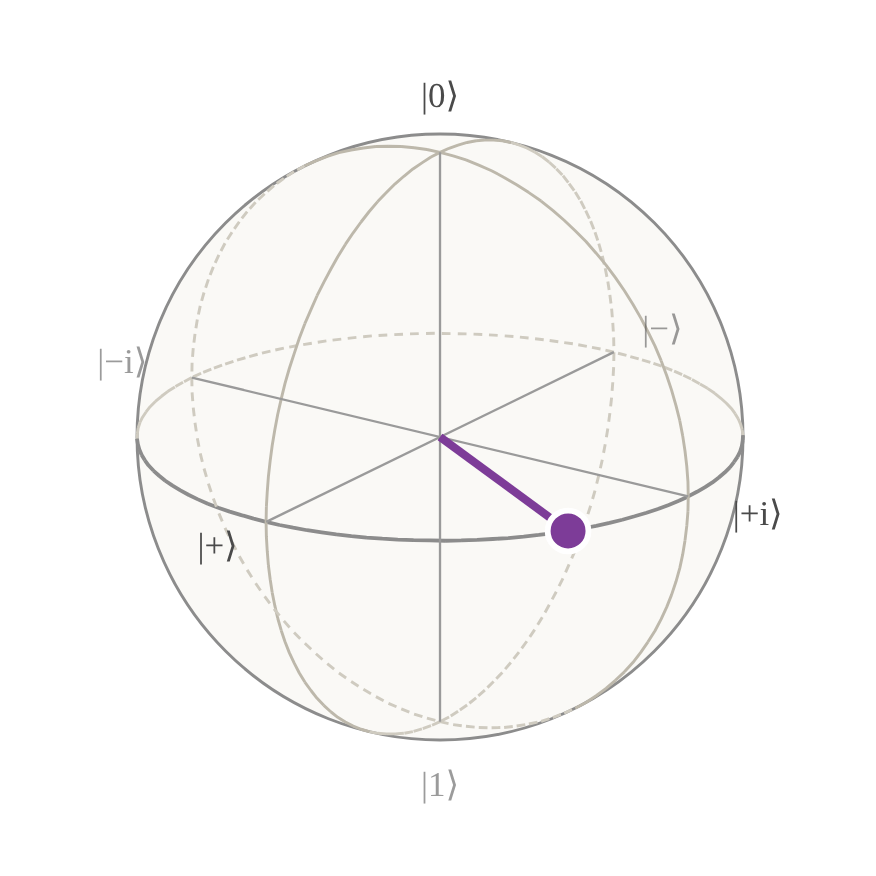
\includegraphics[width=0.66\linewidth]{Imágenes/p12_bloch_ejemplo.png}
\caption{Esfera de Bloch del widget (panel (c)) para el estado del ejemplo, $\alpha=\frac1{\sqrt2}$, $\beta=\frac1{\sqrt2}e^{i\pi/3}$. Su inclinación es $\theta=\frac\pi2$ (está en el ecuador) y su longitud es $\varphi=\frac\pi3$. Los polos son $\ket0$ y $\ket1$, y sobre los ejes del ecuador están $\ket+$ y $\ket{{+}i}$ (con sus opuestos $\ket-$ y $\ket{{-}i}$).}
\label{fig:bloch}
\end{figure}

%======================================================================
\subsection*{De los coeficientes a la esfera: del panel (a) al panel (c)}
%======================================================================

\paragraph{Qué se traduce.}
Se parte de los cuatro números del panel (a), $\alpha=Ae^{ix}$ y $\beta=Be^{iy}$, y se quiere un
punto de la esfera, es decir, dos ángulos: la inclinación $\theta$ y la longitud $\varphi$. Como
la esfera solo guarda los dos datos que no dependen de la fase global, la traducción consiste en
deshacerse de la fase global y escribir los dos datos que quedan como ángulos: el reparto entre
$A$ y $B$ se convierte en $\theta$ y la fase relativa en $\varphi$.

\paragraph{Se quita la fase global.}
Como $e^{ix}e^{-ix}=1$, el coeficiente $\beta$ se puede escribir como
$Be^{iy}=e^{ix}\,Be^{i(y-x)}$, y el factor $e^{ix}$ sale de los dos términos:
\[
  \ket\psi=Ae^{ix}\ket0+Be^{iy}\ket1
  =e^{ix}\bigl(A\ket0+Be^{i(y-x)}\ket1\bigr).
\]
El factor $e^{ix}$ es una fase global, así que $\ket\psi$ se identifica con el estado entre
paréntesis, $A\ket0+Be^{i(y-x)}\ket1$. En ese estado el primer coeficiente es el número real
$A\ge0$, y la única fase que queda es la fase relativa, que se toma como longitud:
\begin{equation}\label{eq:phi}
  \destacado{\varphi\equiv y-x \pmod{2\pi}.}
\end{equation}

\paragraph{El reparto entre $A$ y $B$ se convierte en un ángulo.}
Quedan dos números, $A$ y $B$, pero no son independientes: si se conoce $A$, la condición
$A^2+B^2=1$ y $B\ge0$ dan $B=\sqrt{1-A^2}$. Una manera de describir la pareja con un solo número
es verla como un punto $(A,B)$ del plano. Ese punto está a distancia $\sqrt{A^2+B^2}=1$ del
origen, y como $A,B\ge0$, está en el primer cuadrante, es decir, sobre el cuarto de
circunferencia de la figura~\ref{fig:theta}. Un punto de ese cuarto de circunferencia queda
determinado por el ángulo $\omega\in[0,\frac\pi2]$ que forma con el eje horizontal, y sus
coordenadas son $A=\cos\omega$ y $B=\sin\omega$ (son las coordenadas polares de un punto a
distancia $1$ del origen).

El ángulo $\omega$ mide cómo se reparte la probabilidad: con $\omega=0$ se tiene $A=1$, $B=0$ y
el resultado es $0$ con certeza; con $\omega=\frac\pi2$ se tiene $A=0$, $B=1$ y el resultado es
$1$ con certeza; con $\omega=\frac\pi4$, $A=B=\frac1{\sqrt2}$ y los dos resultados tienen
probabilidad $\frac12$.

Falta ubicar ese reparto en la esfera. La esfera de Bloch pone $\ket0$ en el polo norte, donde
$\theta=0$, y $\ket1$ en el polo sur, donde $\theta=\pi$; se eligen puntos opuestos porque
$\ket0$ y $\ket1$ son ortogonales, $\bk01=0$. Así, cuando $\omega$ va de $0$ a $\frac\pi2$, la
inclinación tiene que ir de $0$ a $\pi$, que es el doble. Por eso se toma $\theta=2\omega$, o
sea, $\omega=\frac\theta2$, y las igualdades $A=\cos\omega$, $B=\sin\omega$ se convierten en
\begin{equation}\label{eq:theta}
  \destacado{\cos\tfrac\theta2=A,\qquad \sin\tfrac\theta2=B .}
\end{equation}
El $\frac12$ en $\frac\theta2$ no es una convención arbitraria: es lo que hace que el cuarto de
circunferencia, que solo abarca un ángulo de $\frac\pi2$, cubra en la esfera todo el camino de
un polo al otro.

\begin{figure}[htbp]
\centering
\begin{tikzpicture}[scale=2.6, line cap=round]
  \draw[-{Stealth[length=2mm]}, black!60] (-0.08,0) -- (1.25,0) node[right, font=\footnotesize]{$A$};
  \draw[-{Stealth[length=2mm]}, black!60] (0,-0.08) -- (0,1.25) node[above, font=\footnotesize]{$B$};
  \draw[very thick, colSd] (1,0) arc[start angle=0, end angle=90, radius=1];
  \draw[thick, black!80] (0,0) -- (0.866,0.5);
  \draw[densely dotted, black!60] (0.866,0.5) -- (0.866,0);
  \draw[densely dotted, black!60] (0.866,0.5) -- (0,0.5);
  \fill[black!85] (0.866,0.5) circle (0.022);
  \node[font=\scriptsize, anchor=south west] at (0.87,0.5) {$(A,B)$};
  \draw[resaltado, thick] (0.28,0) arc[start angle=0, end angle=30, radius=0.28];
  \node[resaltado, font=\scriptsize, anchor=west] at (0.30,0.055) {$\omega=\frac\theta2$};
  \node[font=\scriptsize, anchor=north] at (0.866,0) {$\cos\frac\theta2$};
  \node[font=\scriptsize, anchor=east] at (0,0.5) {$\sin\frac\theta2$};
  \fill[colCu] (1,0) circle (0.025);
  \node[colCu, font=\scriptsize, anchor=north west] at (1,0) {$\ket0$: $A=1$};
  \fill[colSu] (0,1) circle (0.025);
  \node[colSu, font=\scriptsize, anchor=south west] at (0.02,1.0) {$\ket1$: $B=1$};
  \node[font=\scriptsize, anchor=north] at (0.5,-0.2) {$\omega$ va de $0$ a $\frac\pi2$};
\end{tikzpicture}

\caption{El punto $(A,B)$ está sobre un cuarto de circunferencia y queda determinado por el ángulo $\omega$. De $\ket0$ a $\ket1$, el ángulo $\omega$ recorre solo $\frac\pi2$. En la esfera de Bloch, en cambio, la inclinación $\theta$ va de $\ket0$ (polo norte) a $\ket1$ (polo sur) y recorre $\pi$, el doble. Por eso $\theta=2\omega$, de modo que $A=\cos\frac\theta2$ y $B=\sin\frac\theta2$.}
\label{fig:theta}
\end{figure}

La tabla siguiente muestra los tres casos de referencia.
\[
\renewcommand{\arraystretch}{1.35}
\begin{array}{c|c|c|c|l}
A & B & \omega=\theta/2 & \theta & \text{Posición en la esfera}\\ \hline
1 & 0 & 0 & 0 & \text{polo norte, } \ket0\\
\frac1{\sqrt2} & \frac1{\sqrt2} & \frac\pi4 & \frac\pi2 & \text{ecuador}\\
0 & 1 & \frac\pi2 & \pi & \text{polo sur, } \ket1
\end{array}
\]

\paragraph{Fórmula.}
Al reunir $\varphi\equiv y-x$ y $\cos\frac\theta2=A$, $\sin\frac\theta2=B$, el estado entre
paréntesis se escribe con los dos ángulos, y salvo fase global, todo estado tiene la forma
\begin{equation}\label{eq:forma-bloch}
  \ket\psi\sim\cos\tfrac\theta2\,\ket0+e^{i\varphi}\sin\tfrac\theta2\,\ket1,
  \qquad \theta\in[0,\pi],\ \varphi\in(-\pi,\pi] ,
\end{equation}
que es la forma con la que la esfera de Bloch se presenta en la bibliografía del curso (Nielsen
y Chuang, sección~1.2).

El punto también se puede calcular sin pasar por los ángulos. Con $\cos\frac\theta2=A$,
$\sin\frac\theta2=B$ y $\varphi\equiv y-x$ se tiene
$\overline\alpha\beta=Ae^{-ix}Be^{iy}=AB\,e^{i(y-x)}=\cos\frac\theta2\sin\frac\theta2\,e^{i\varphi}$,
y por las fórmulas del ángulo doble, $2\sin\frac\theta2\cos\frac\theta2=\sin\theta$ y
$\cos^2\frac\theta2-\sin^2\frac\theta2=\cos\theta$. Por tanto,
$2\overline\alpha\beta=\sin\theta\,e^{i\varphi}=\sin\theta\cos\varphi+i\sin\theta\sin\varphi$ y
$A^2-B^2=\cos\theta$. Con la notación del punto 1.1, en la que $\Real z=a$ es la parte real e $\Imag z=b$ la parte imaginaria de $z=a+ib$, se obtiene
\begin{equation}\label{eq:a-c}
  \destacado{\vec r=(\sin\theta\cos\varphi,\ \sin\theta\sin\varphi,\ \cos\theta)
  =\bigl(2\Real(\overline\alpha\beta),\ 2\Imag(\overline\alpha\beta),\ A^2-B^2\bigr).}
\end{equation}
Es decir, se calcula el número complejo $2\overline\alpha\beta$: su parte real es la coordenada $r_x$ del punto y su parte imaginaria es la coordenada $r_y$. En el ejemplo, $2\overline\alpha\beta=2\cdot\frac1{\sqrt2}\cdot\frac1{\sqrt2}e^{i\pi/3}=e^{i\pi/3}=\frac12+i\frac{\sqrt3}{2}$, así que $r_x=\frac12$, $r_y=\frac{\sqrt3}{2}$ y $r_z=\frac12-\frac12=0$.
Esta segunda expresión no usa las fases $x$ y $y$, así que sigue siendo válida cuando $A=0$ o
$B=0$, que es justamente cuando alguna fase no está determinada. En esos casos $\sin\theta=0$ y
el punto está en uno de los polos, de modo que $\varphi$ no hace falta.

\paragraph{Qué significa.}
La altura del punto en la esfera es $r_z=\cos\theta=A^2-B^2$, la diferencia entre la
probabilidad de obtener $0$ y la de obtener $1$. Dicho de otra forma, $r_z$ es el valor esperado de una medición que vale $+1$ si el resultado es $0$ y $-1$ si es $1$: el punto está en
el polo norte cuando el resultado es $0$ con certeza, en el polo sur cuando es $1$ con certeza y
en el ecuador cuando los dos resultados son igualmente probables. La longitud $\varphi$, en
cambio, no se ve en esas probabilidades; es la fase relativa, que no tiene análogo en una moneda clásica con probabilidades $|\alpha|^2$ y $|\beta|^2$. Por ejemplo, $\ket+$ y $\ket-$ están ambos en el ecuador
($\theta=\frac\pi2$), pero en lados opuestos ($\varphi=0$ y $\varphi=\pi$). En el ejemplo,
$A=B=\frac1{\sqrt2}$ da $\cos\theta=\frac12-\frac12=0$, es decir, $\theta=\frac\pi2$ (el
ecuador), y $\varphi=\frac\pi3-0=\frac\pi3$.

%======================================================================
\subsection*{De la esfera a los coeficientes: del panel (c) al panel (a)}
%======================================================================

\paragraph{Qué se traduce.}
Se parte de un punto de la esfera, es decir, de dos ángulos $\theta$ y $\varphi$, y se quieren
dos números complejos. La esfera no guarda la fase global, así que esta traducción no tiene una
única respuesta: a cada punto le corresponde toda una familia de parejas $(\alpha,\beta)$, y
para obtener una hay que elegir la fase global.

\paragraph{Fórmula.}
Por la forma~$\ket\psi\sim\cos\tfrac\theta2\,\ket0+e^{i\varphi}\sin\tfrac\theta2\,\ket1$ \eqref{eq:forma-bloch},
$\ket\psi\sim\cos\frac\theta2\ket0+e^{i\varphi}\sin\frac\theta2\ket1$, el estado
$\cos\frac\theta2\ket0+e^{i\varphi}\sin\frac\theta2\ket1$ corresponde al punto, y todos los demás
difieren de él en una fase global $e^{i\gamma}$. Al multiplicar los dos coeficientes por
$e^{i\gamma}$ se obtiene
\begin{equation}\label{eq:c-a}
  \destacado{\alpha=e^{i\gamma}\cos\tfrac\theta2,\qquad
  \beta=e^{i(\gamma+\varphi)}\sin\tfrac\theta2,\qquad \gamma\in\mathbb R\text{ arbitrario},}
\end{equation}
es decir, $A=\cos\frac\theta2$, $x=\gamma$, $B=\sin\frac\theta2$ y $y=\gamma+\varphi$.

\paragraph{Qué significa.}
Las dos primeras igualdades deshacen las de la traducción anterior: $A=\cos\frac\theta2$ y
$B=\sin\frac\theta2$ recuperan los módulos, y $y-x=(\gamma+\varphi)-\gamma=\varphi$ recupera la
fase relativa. El ángulo $\gamma$ es la fase global elegida. Cambiarlo gira los dos puntos del
panel (a) el mismo ángulo alrededor del origen, como en la figura~\ref{fig:fases}, sin moverlos
del punto de la esfera. En el widget, $\gamma$ se controla con un deslizador que fija
$x=\gamma$.

%======================================================================
\subsection*{De la onda a la esfera: del panel (b) al panel (c)}
%======================================================================

\paragraph{Qué se traduce.}
Se parte de las ondas del panel (b) y se quiere un punto de la esfera. La traducción es la
composición de dos de las anteriores: de las ondas se pasa a los coeficientes leyendo las
crestas, y de los coeficientes a la esfera con $\cos\frac\theta2=A$, $\sin\frac\theta2=B$ y
$\varphi\equiv y-x$.

\paragraph{Fórmula.}
Por la ecuación~$A=\text{altura de }\alpha\ket0,\quad\penalty0 x\equiv t_\alpha,\quad\penalty0 B=\text{altura de }\beta\ket1,\quad\penalty0 y\equiv 2t_\beta$ \eqref{eq:b-a}, $A$ y $B$ son las alturas de las ondas, $x\equiv t_\alpha$ y
$y\equiv 2t_\beta$. Al sustituir estos valores en $\cos\theta=A^2-B^2$ y en
$\varphi\equiv y-x$, los ángulos de la esfera quedan escritos directamente en términos de las
ondas:
\begin{equation}\label{eq:b-c}
  \destacado{\cos\theta=(\text{altura de }\alpha\ket0)^2-(\text{altura de }\beta\ket1)^2,
  \qquad \varphi\equiv 2t_\beta-t_\alpha \pmod{2\pi}.}
\end{equation}

\paragraph{Qué significa.}
La inclinación depende solo de las alturas y la longitud solo de las posiciones de las crestas.
La primera igualdad dice que la altura del punto en la esfera mide cómo se reparte la norma entre
la frecuencia $1$ y la frecuencia $2$: si toda la norma está en $\cos t$, el punto está en el
polo norte, y si toda está en $\cos 2t$, en el polo sur. La segunda dice que la longitud mide el
desfase entre las crestas, pero contado en la escala de la frecuencia $2$; no es la simple
diferencia $t_\beta-t_\alpha$, porque una misma distancia en $t$ corresponde a un ángulo doble en
la onda de frecuencia $2$. En el ejemplo de la figura~\ref{fig:a-b}, ambas alturas son
$\frac1{\sqrt2}$, así que $\cos\theta=0$, y $\varphi=2\cdot\frac\pi6-0=\frac\pi3$, el mismo punto
obtenido desde el panel (a).

%======================================================================
\subsection*{De la esfera a la onda: del panel (c) al panel (b)}
%======================================================================

\paragraph{Qué se traduce.}
Se parte de un punto de la esfera y se quiere una función de $t$. Es la composición de la
traducción de (c) a (a) con la de (a) a (b), y, como la primera, requiere elegir la fase
global.

\paragraph{Fórmula.}
Por la ecuación~$\alpha=e^{i\gamma}\cos\tfrac\theta2,\quad\penalty0 \beta=e^{i(\gamma+\varphi)}\sin\tfrac\theta2$ \eqref{eq:c-a}, $A=\cos\frac\theta2$, $x=\gamma$, $B=\sin\frac\theta2$ y
$y=\gamma+\varphi$. Al sustituir estos valores en la onda de la ecuación~$\alpha\ket0=A\cos(t-x),\quad\penalty0 \beta\ket1=B\cos(2t-y),\quad\penalty0 \psi(t)=A\cos(t-x)+B\cos(2t-y)$ \eqref{eq:a-b},
$\psi(t)=A\cos(t-x)+B\cos(2t-y)$, se obtiene
\begin{equation}\label{eq:c-b}
  \destacado{\psi(t)=\cos\tfrac\theta2\,\cos(t-\gamma)
  +\sin\tfrac\theta2\,\cos(2t-\gamma-\varphi).}
\end{equation}

\paragraph{Qué significa.}
Un mismo punto de la esfera corresponde a toda una familia de ondas, una para cada $\gamma$, y
esas ondas no son simples copias corridas unas de otras, como se explica a continuación.

%======================================================================
\subsection*{Fase global y desplazamientos en el tiempo}
%======================================================================

La onda $\psi(t)=\cos\frac\theta2\cos(t-\gamma)+\sin\frac\theta2\cos(2t-\gamma-\varphi)$ de la
ecuación~$\psi(t)=\cos\tfrac\theta2\,\cos(t-\gamma)+\sin\tfrac\theta2\,\cos(2t-\gamma-\varphi)$ \eqref{eq:c-b} muestra un hecho que el widget permite ver directamente. Al cambiar la
fase global $\gamma$, la onda $\alpha\ket0=\cos\frac\theta2\cos(t-\gamma)$ se corre $\gamma$
hacia la derecha, mientras que
$\beta\ket1=\sin\frac\theta2\cos\bigl(2(t-\frac{\gamma+\varphi}2)\bigr)$ se corre solo
$\gamma/2$. Como las dos componentes se corren distancias distintas, la suma $\psi$ cambia de
forma, aunque el punto de Bloch sea el mismo (figura~\ref{fig:fase-global}, izquierda).

Un desplazamiento en el tiempo produce el efecto contrario. Si $\psi(t)$ se reemplaza por
$\psi(t-\tau)$, la componente $A\cos(t-\tau-x)$ pasa a tener fase $x+\tau$ y la componente
$B\cos(2t-2\tau-y)$ pasa a tener fase $y+2\tau$; es decir, $\alpha$ se multiplica por
$e^{i\tau}$ y $\beta$ por $e^{2i\tau}$. Como los dos coeficientes no se multiplican por el mismo
número, esto no es una fase global. Los módulos no cambian, así que $\theta$ tampoco, pero la
longitud $\varphi\equiv y-x$ pasa a ser $(y+2\tau)-(x+\tau)=\varphi+\tau$: correr la onda en el
tiempo hace girar el punto de Bloch un ángulo $\tau$ alrededor del eje $z$
(figura~\ref{fig:fase-global}, derecha).

\begin{figure}[htbp]
\centering
\begin{tikzpicture}
\begin{axis}[ondaT, ymin=-1.6, ymax=1.75,
  title={Misma posición en la esfera: $\gamma=0$ y $\gamma=\pi/2$}]
  \addplot[very thick, black!85] {0.7071*cos(x)+0.7071*cos(2*x-pi/3)};
  \addplot[very thick, colSd, densely dashed] {0.7071*cos(x-pi/2)+0.7071*cos(2*x-pi/2-pi/3)};
  \node[font=\footnotesize, anchor=west] at (axis cs:4.5,1.55) {$\gamma=0$};
  \draw[very thick, black!85] (axis cs:3.9,1.55) -- (axis cs:4.45,1.55);
  \node[font=\footnotesize, anchor=west, colSd] at (axis cs:4.5,1.25) {$\gamma=\frac{\pi}{2}$};
  \draw[very thick, colSd, densely dashed] (axis cs:3.9,1.25) -- (axis cs:4.45,1.25);
\end{axis}
\end{tikzpicture}
\hfill
\begin{tikzpicture}
\begin{axis}[ondaT, ymin=-1.6, ymax=1.75,
  title={Desplazamiento en el tiempo: $\psi(t)$ y $\psi(t-\frac{\pi}{2})$}]
  \addplot[very thick, black!85] {0.7071*cos(x)+0.7071*cos(2*x-pi/3)};
  \addplot[very thick, resaltado, densely dashed] {0.7071*cos(x-pi/2)+0.7071*cos(2*x-pi-pi/3)};
  \node[font=\footnotesize, anchor=west] at (axis cs:4.5,1.55) {$\psi(t)$};
  \draw[very thick, black!85] (axis cs:3.9,1.55) -- (axis cs:4.45,1.55);
  \node[font=\footnotesize, anchor=west, resaltado] at (axis cs:4.5,1.25) {$\psi(t-\frac{\pi}{2})$};
  \draw[very thick, resaltado, densely dashed] (axis cs:3.9,1.25) -- (axis cs:4.45,1.25);
\end{axis}
\end{tikzpicture}
\caption{Ambos paneles parten del estado con $\theta=\pi/2$, $\varphi=\pi/3$. A la izquierda, al
cambiar la fase global de $0$ a $\pi/2$ la onda cambia de forma, pero el punto de Bloch no se
mueve. A la derecha, la misma onda corrida $\pi/2$ en el tiempo conserva su forma, pero su
punto de Bloch gira $\pi/2$ alrededor del eje $z$, de $\varphi=\pi/3$ a $\varphi=5\pi/6$.}
\label{fig:fase-global}
\end{figure}

%======================================================================
\subsection*{Resumen de las seis traducciones}
%======================================================================

Con $\alpha=Ae^{ix}$, $\beta=Be^{iy}$, $A^2+B^2=1$, las fórmulas deducidas son las siguientes.
\[
\renewcommand{\arraystretch}{1.6}
\begin{array}{l|l}
\text{Traducción} & \text{Fórmula}\\ \hline
\text{(a)}\to\text{(b)} & \psi(t)=A\cos(t-x)+B\cos(2t-y)\\
\text{(b)}\to\text{(a)} & A=\text{altura de }\alpha\ket0,\ \ x\equiv t_\alpha,\ \
  B=\text{altura de }\beta\ket1,\ \ y\equiv 2t_\beta\\
\text{(a)}\to\text{(c)} & \cos\frac\theta2=A,\ \ \sin\frac\theta2=B,\ \ \varphi\equiv y-x
  \quad\bigl(\vec r=(2\Real\overline\alpha\beta,\ 2\Imag\overline\alpha\beta,\ A^2-B^2)\bigr)\\
\text{(c)}\to\text{(a)} & \alpha=e^{i\gamma}\cos\frac\theta2,\ \
  \beta=e^{i(\gamma+\varphi)}\sin\frac\theta2,\ \ \gamma \text{ libre}\\
\text{(b)}\to\text{(c)} & \cos\theta=(\text{altura de }\alpha\ket0)^2-(\text{altura de }\beta\ket1)^2,\ \
  \varphi\equiv 2t_\beta-t_\alpha\\
\text{(c)}\to\text{(b)} & \psi(t)=\cos\frac\theta2\cos(t-\gamma)+\sin\frac\theta2\cos(2t-\gamma-\varphi)
\end{array}
\]

%======================================================================
\subsection*{Implementación}
%======================================================================

El widget guarda el estado como los cuatro números $A$, $x$, $B$ y $y$ de la forma polar
$\alpha=Ae^{ix}$, $\beta=Be^{iy}$, en lugar de $\alpha$ y $\beta$ directamente, para no perder la
fase de un coeficiente cuando su módulo se hace cero. Cada interacción modifica estos números y
luego redibuja los tres paneles con las fórmulas anteriores. Al arrastrar $\alpha$ en el
panel (a), $A$ y $x$ pasan a ser el módulo y el ángulo del punto, y $B$ se ajusta a
$\sqrt{1-A^2}$ sin cambiar $y$; lo mismo ocurre al arrastrar $\beta$. Al arrastrar una cresta en
el panel (b), la altura fija el módulo y la posición fija la fase, según
$x\equiv t_\alpha$ y $y\equiv 2t_\beta$. Las ondas se dibujan con
$\psi(t)=A\cos(t-x)+B\cos(2t-y)$ y el punto de Bloch con
$\vec r=\bigl(2\Real(\overline\alpha\beta),\ 2\Imag(\overline\alpha\beta),\ A^2-B^2\bigr)$. El
notebook de Python del repositorio comprueba numéricamente las fórmulas de esta sección. Para eso genera doscientos estados al azar: para cada uno sortea las partes reales e imaginarias de $\alpha$ y $\beta$ y después divide entre la norma, de modo que $|\alpha|^2+|\beta|^2=1$. Con cada estado verifica que cada fórmula de ida se invierte con su fórmula de vuelta (al pasar por la esfera, salvo fase global), así como las propiedades de la fase global y de los desplazamientos en el tiempo descritas en la sección anterior. Si alguna igualdad fallara, el programa se detendría con un error. Esta comprobación no reemplaza las deducciones anteriores: sirve para detectar errores en las fórmulas o en el código.